\documentclass[notheorems]{beamer}

\setbeamertemplate{theorem}[ams style]
\setbeamertemplate{theorems}[numbered]

% ----- Latex properties
\usepackage[latin1]{inputenc}
\usepackage{tikz} % 2D drawing
\usepackage{graphicx} % enhanced graphics
\graphicspath{ {./img/} {./} }

% ----- Beamer theme properties
\usetheme[left,hideothersubsections]{Goettingen}
\usecolortheme{crane,sidebartab}
\usefonttheme{structureitalicserif}
\useinnertheme[shadow]{rounded}
\setbeamercovered{transparent}

\theoremstyle{definition}
\newtheorem{researchquestion}{Question}
\newtheorem{definition}{Definition}
\newtheorem{answer}{Answer to question}

\theoremstyle{example}
\newtheorem{example}{Example}
\newtheorem{recommendation}{Recommendation}



% ----- Document properties
\title[Statistical Properties of DKD]
{%
Investigating the Statistical Properties\\
of the Double Kernel Density Estimator
}
\author[Harold Ship]
{%
    Harold~Ship
    \\
    {%
    \tiny
    THESIS SUBMITTED IN PARTIAL FULFILLMENT OF THE REQUIREMENTS FOR THE MASTER'S DEGREE
    }
    \\
    {%
    \small
    Advisors: Prof.~Boris~Portnov \and
    Dr.~Itai~Dattner \and
    Prof.~Em.~Benjamin~Reiser
    }
}
\institute[University~of~Haifa]
{%
University~of~Haifa \and 
Faculty~of~Management \and
Department~of~Information~\&~Knowledge~Management
}

\date{January 30, 2019}

%
% ----- The presentation
%
\begin{document}

% ----- Title page
\begin{frame}
\tikz [remember picture,overlay]
    \node at
        ([xshift=0.9cm, yshift=-3.6cm]current page.west) 
        {
\includegraphics[width=1.5cm]{univ_logo2.png}};
    \titlepage
\end{frame}

% ----- SECTION: Introduction
\section*{Introduction}

\begin{frame}\frametitle{Mapping disease incidence}
    \begin{center}{ 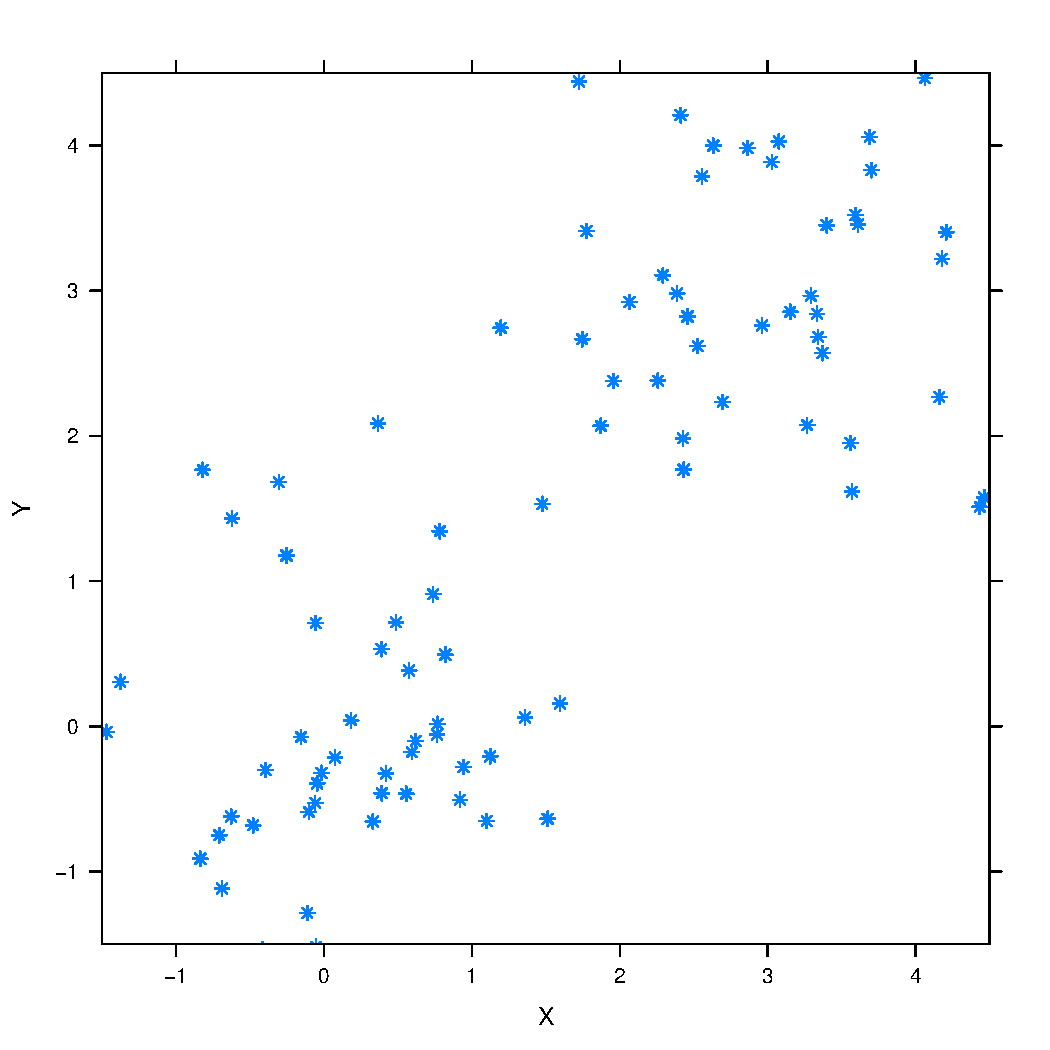
\includegraphics[width=0.5\textwidth]{example-incidents} }\end{center}
    \begin{itemize}
        \item Is there a pattern here?
        \item Does it simply reflect population density?
        \item Or is the risk of disease higher in some locations?
    \end{itemize}
\end{frame}

\begin{frame}\frametitle{How can we tell?}
    We need a tool that:
    \begin{itemize}
        \item allows us to compare the risk at different locations
        \item can find areas of high risk
        \item can do so accurately
    \end{itemize}
\end{frame}

\begin{frame}\frametitle{The double kernel density}
    \begin{itemize}
        \item The \emph{double kernel density} (DKD) has been used in the literature \cite{kloog2009using}, \cite{portnov2009studying}, \cite{zusman2012residential}
        \item The statistical properties of the DKD have not been studied
        \item This research:
        \begin{itemize}
            \item Looks to build a methodological framework for studying some of the statistical properties
            \item Methodology will be based on computer simulations of the stochastic process of disease incidence
            \item Will assess the performance of the DKD method
        \end{itemize}
    \end{itemize}
\end{frame}

% ----- Outline
\begin{frame}{Outline}
\tableofcontents[hideallsubsections]
\end{frame}

% ----- SECTION: Theoretical background
\section{Theoretical background}

% ----- SUBSECTION: Measuring disease risk
\subsection{Measuring disease risk}
\begin{frame}\frametitle{Measuring disease risk}
    \begin{itemize}
        \item How do I measure the risk of developing a disease?
        \item How do I compare the problem of disease in different times and places?
    \end{itemize}
    \begin{definition}
        \alert{Cumulative incidence} or \alert{risk} is the proportion of the at-risk population that develop a disease during the study period.
        \begin{equation*}
            \lambda = \frac{number~of~new~cases~of~disease}{number~of~people~who~can~get~it}
        \end{equation*}
        \cite{bonita2006basic}
    \end{definition}
    \begin{itemize}
        \item We are interested in comparing the risk at different \emph{locations}, represented by $(x,y)$ coordinates
    \end{itemize}
\end{frame}

% ----- SUBSECTION: Smoothing disease cases
\subsection{Smoothing disease cases}
\begin{frame}\frametitle{Smoothing disease cases}
    \begin{itemize}
        \item Are cases of disease concentrated in specific areas?
        \item Administrative boundaries: problematic
            \begin{itemize}
                \item Arbitrary boundaries
                \item Heterogenous populations
                \item Small number of cases: privacy
            \end{itemize}
        \item \alert{Kernel smoothing} to compute \emph{intensity} a.k.a \emph{density}
        \item Accuracy is highly dependent on the \emph{bandwidth} \textbf{(h)} which controls the amount of smoothing
    \end{itemize}
    \begin{example}{\tiny{\textbf{Left:} case locations, smoothed with \textbf{Middle:} small value of \emph{h}. \textbf{Right:} large value of \emph{h}.}}
    \centerline{
        \label{fig:points-and-dkd}
        \centering
        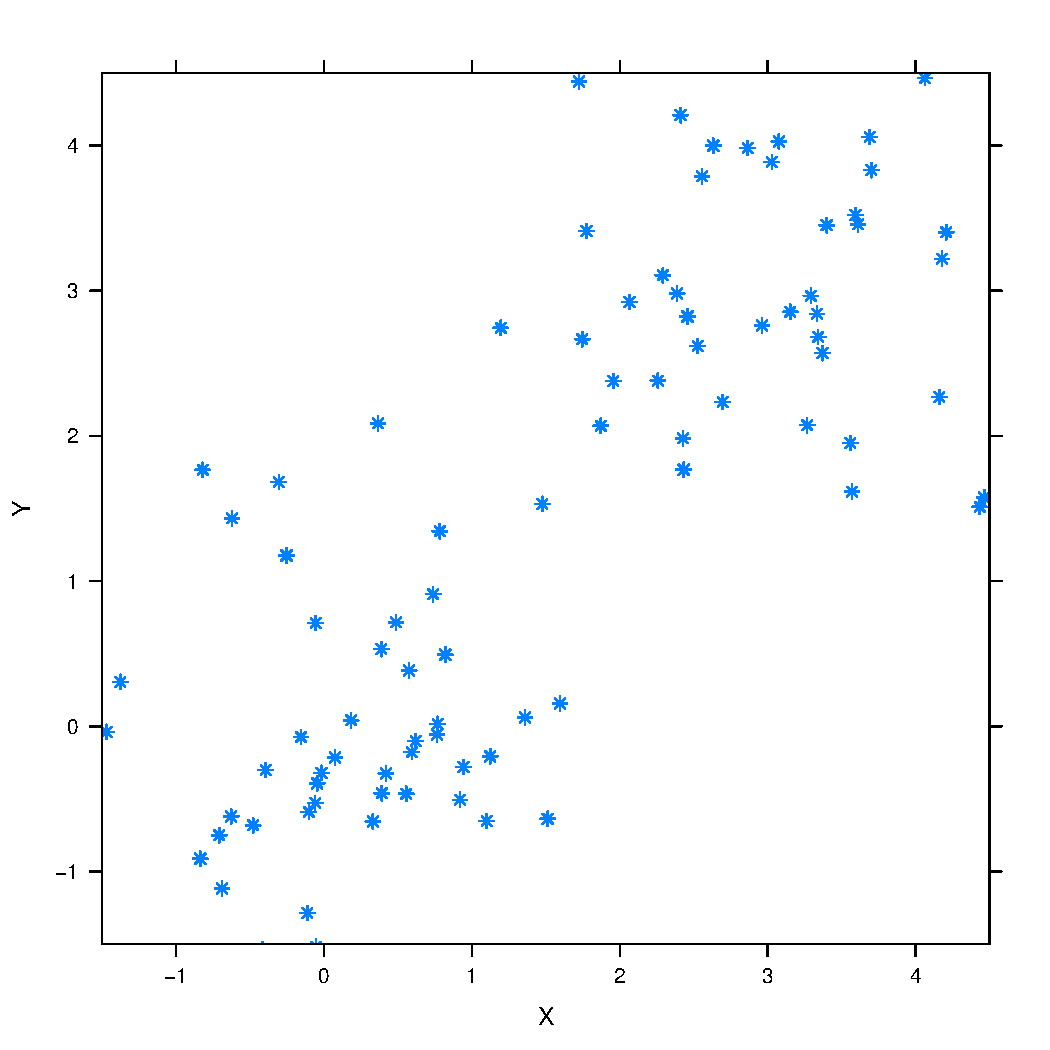
\includegraphics[width=0.3\textwidth]{example-incidents}
        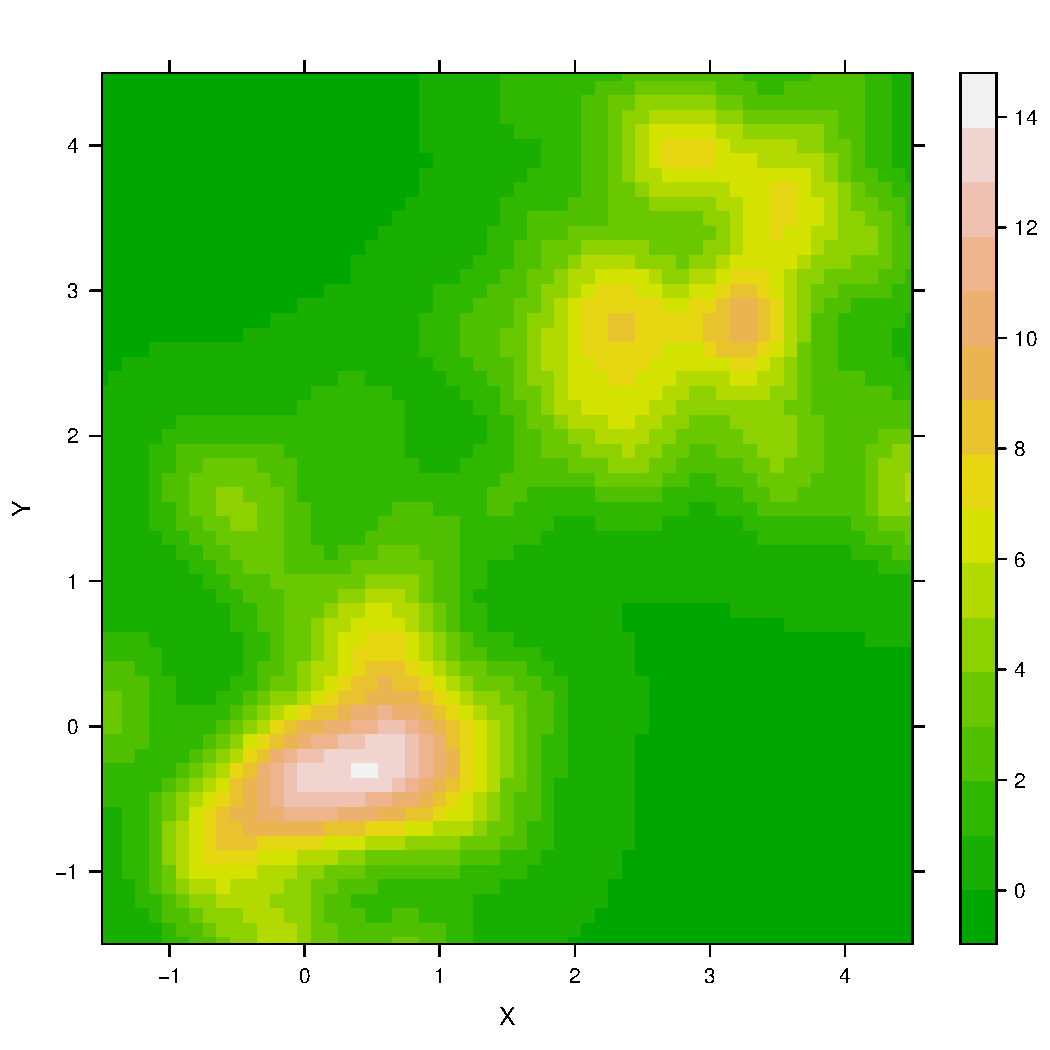
\includegraphics[width=0.3\textwidth]{example-incidents-undersmoothed}
        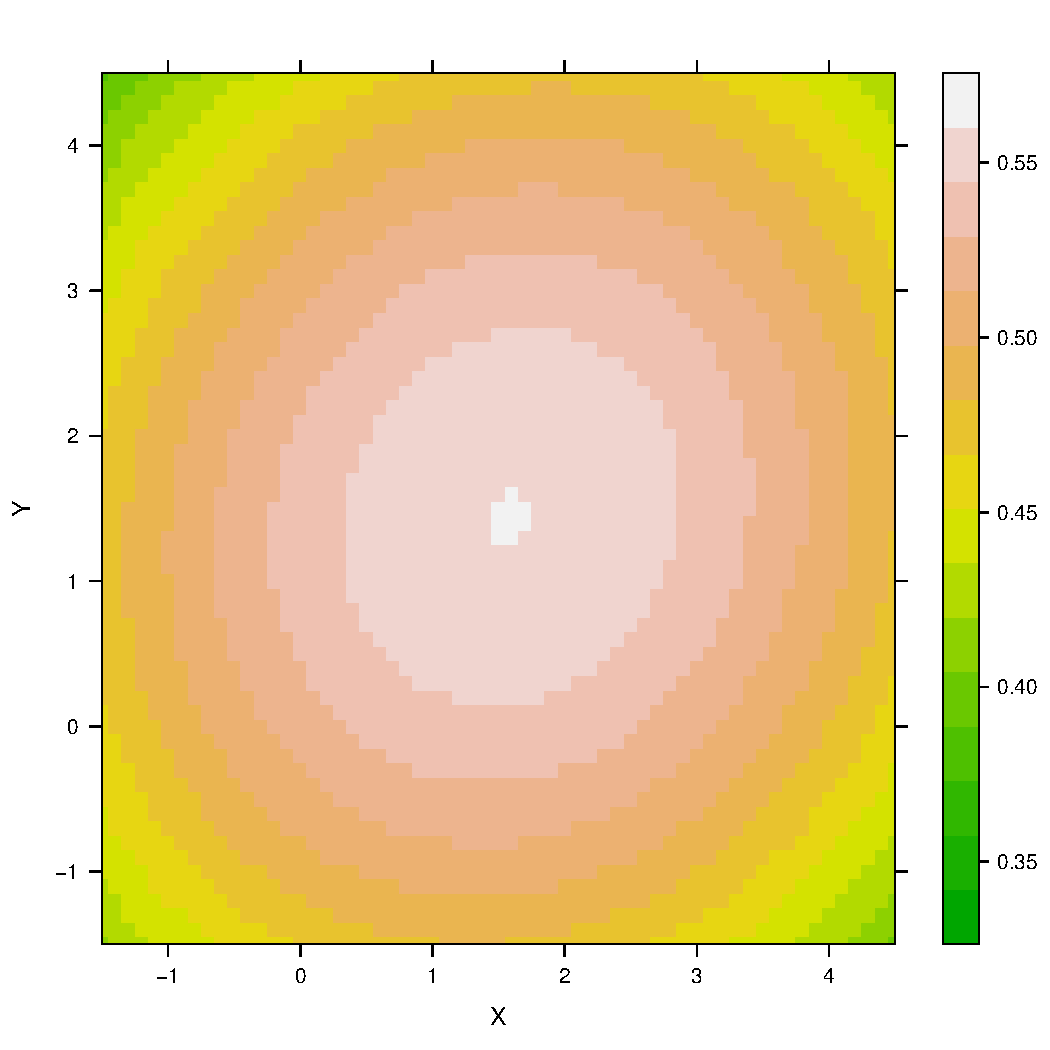
\includegraphics[width=0.3\textwidth]{example-incidents-oversmoothed}
    }
    \end{example}
\end{frame}

% ----- SUBSECTION: Estimating disease risk with the double kernel density
\subsection{Estimating disease risk with the double kernel density}
\begin{frame}\frametitle{Estimating disease risk with the double kernel density}
    \begin{itemize}
        \item We want to know $\lambda$, the risk of developing disease, at a point $(x_1,x_2)$
        \item Smooth the cases and the population separately
        \item Divide to get a function \textbf{$\hat{\lambda}$} that \emph{estimates} the risk at any point
    \end{itemize}
    \begin{definition}
        The \alert{double kernel density} estimator is computed at a point by dividing the \emph{disease case intensity} by the \emph{population intensity} at that point.
        \begin{equation*}
            \hat{\lambda}_{dkd}(x_1,x_2;h) = \frac{ \hat{\lambda}_{I}(x_1,x_2;h) } { \hat{\lambda}_{P}(x_1,x_2;h) }
        \end{equation*}
    \end{definition}
\end{frame}

% ----- SUBSECTION: Effect of the bandwidth
\subsection{Effect of the bandwidth}
\begin{frame}\frametitle{Effect of the bandwidth}
    When the bandwidth is:
    \begin{itemize}
        \item too large (R), important details may be lost
        \item too small (L), noise may produce artifacts
        \item just right (C) best estimate
    \end{itemize}
    \begin{example}{\tiny{\textbf{Left:} $h=0.2$ \textbf{Middle:} $h=0.4$ \textbf{Right:} $h=0.8$ }}
    \centerline{
        \label{fig:points-and-dkd}
        \centering
        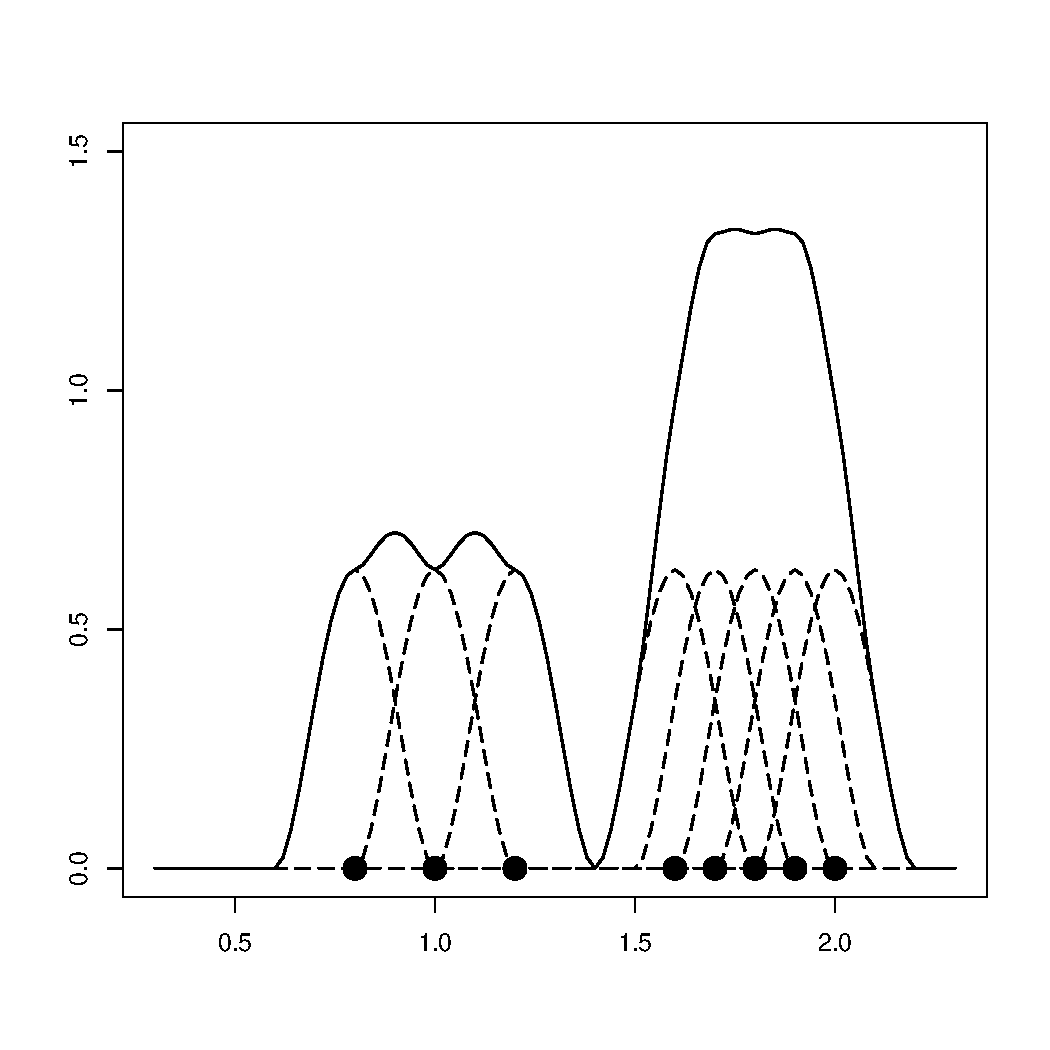
\includegraphics[width=0.3\textwidth]{kernel1d-02}
        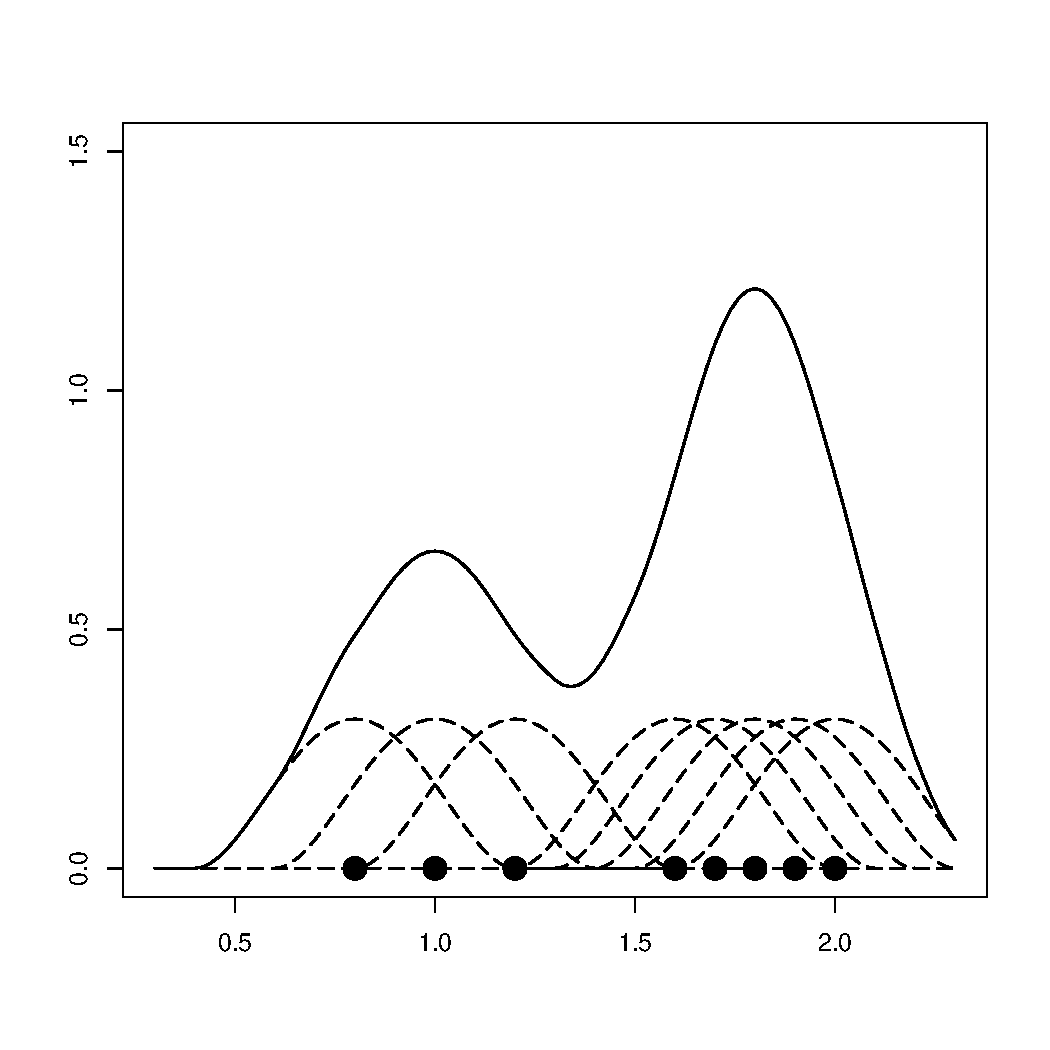
\includegraphics[width=0.3\textwidth]{kernel1d-04}
        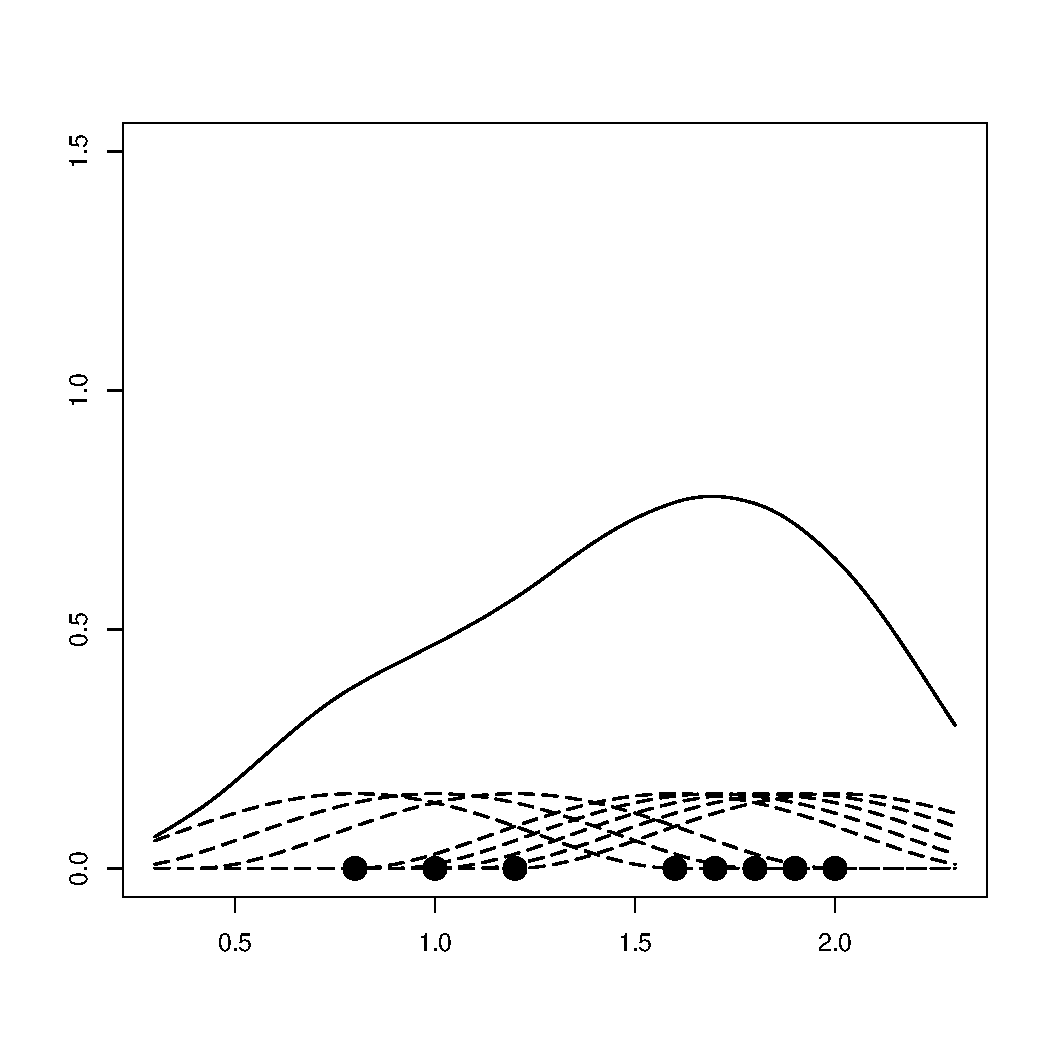
\includegraphics[width=0.3\textwidth]{kernel1d-08}
    }
    \end{example}
\end{frame}

% ----- SUBSECTION: Choosing the bandwidth
\subsection{Choosing the bandwidth}
\begin{frame}\frametitle{Choosing the bandwidth}
    \small
    There are many schemes, we use 3 (well, 2 plus Oracle)
    \begin{definition}
        \textbf{Oracle bandwidth} minimizes the empirical MISE,
        computed from the data samples generated from the true intensity function.
        Needs to know the ``truth''.
    \end{definition}
    \begin{definition}
        \textbf{Silverman's Rule of Thumb bandwidth} $h_S = 2.04~\sigma~n^{-1/6}$
    \end{definition}
    \begin{definition}
        \textbf{Least Squares Cross Validation (CV) bandwidth} uses leave-one-out cross validation to minimize the CV error.
            Choose the pair of bandwidths $h_{x_1}, h_{x_2}$ that minimizes the CV error.
            Asymptotically in $n$, the bandwidth that minimizes MISE also minimizes CV error which can be computed without knowing the ``truth''.
    \end{definition}
\end{frame}

% ----- SECTION: Study goal
\section{Study goal}

% ----- SUBSECTION: Study goal
\subsection{Study goal}
\begin{frame}\frametitle{Study goal}
    \begin{enumerate}
        \item The goal of this study is to examine the statistical properties of the DKD
        \item Can we infer the \emph{risk} function from the data?
        \item If so, how ``good'' a job will the DKD do?
        \item We empirically analyze how different factors affect the accuracy of the DKD
        \item The DKD method can be used to estimate a rate,
            in cases where a set of incident locations and a corresponding set of population locations are available 
    \end{enumerate}
\end{frame}

% ----- SUBSECTION: Research questions
\subsection{Research questions}
\begin{frame}\frametitle{Research questions}
    \begin{researchquestion}{How is the accuracy of the DKD affected by:}
        \begin{enumerate}[a)]
            \item the duration of the study, \label{thm:accuracy-affected:duration}%
            \item different rate functions, \label{thm:accuracy-affected:rates}%
            \item the size of the population, \label{thm:accuracy-affected:popsize}%
            \item and different population distributions. \label{thm:accuracy-affected:popdist}%
        \end{enumerate}
    \end{researchquestion}
    \begin{researchquestion}{When looking at the the factors in Question 1,
    how accurate is the DKD:}
        \begin{enumerate}[a)]
            \item globally, over the study area as a whole, \label{thm:accuracy-scale:global}%
            \item in magnitude, point-wise at the peaks, \label{thm:accuracy-scale:peaks}%
            \item location of the peaks. \label{thm:accuracy-scale:peaks-location}%
        \end{enumerate}
    \end{researchquestion}
\end{frame}

% ----- SECTION: Methodology
\section{Methodology}

% ----- SUBSECTION: Monte Carlo simulations of DKD
\subsection{Monte Carlo simulations of DKD}
\begin{frame}\frametitle{Monte Carlo simulations of DKD}
    \begin{itemize}
        \item Stochastic model of disease incidence
        \item Start with the ``truth'' -- known risk function $\lambda(x_1, x_2)$ over the study area
        \item Simulation: generate a random sample of points (cases)
        \item Compute the DKD from the sample
        \item Compare it to the ``truth''
        \item Repeat \textellipsis
        \item Then compute the different measures of error and take the empirical average
    \end{itemize}
\end{frame}

% ----- SUBSECTION: Measuring the accuracy
\subsection{Measuring the accuracy}
\begin{frame}\frametitle{Measuring the accuracy}
    \begin{itemize}
        \item Mean Integrated Absolute Error (MIAE) -- average absolute error over study area
        \item Mean Integrated Squared Error (MISE) -- similar to MIAE but has theoretical uses
        \item Supremum Error -- average of the worst case
        \item Peak bias -- error in the height of the peak
        \item Peak drift -- distance from true peak to peak of the estimate
        \item Centroid is the center point of the top 5\% of the estimated values
        \item Centroid bias is measured by subtracting the true peak from the estimated value at the centroid
        \item Centroid drift is the distance from true peak to the centroid
    \end{itemize}
\end{frame}

% ----- SUBSECTION: Experimental structure
\subsection{Experimental structure}
\begin{frame}\frametitle{Experimental structure}
    \begin{enumerate}
        \item Define the study area $W$ with buffer
        \item Generate a population $P$ of size $N_p$ using chosen population distribution
        \item Generate the \textbf{true} incident risk function $\lambda(x_1, x_2)$
        \item Compute the Oracle bandwidths $h_o1$, $h_o2$
        \item Do 1,00 simulations and compute errors
    \end{enumerate}
\end{frame}

% ----- SUBSECTION: Main simulations
\subsection{Main simulations}
\begin{frame}\frametitle{Main simulations}
    \begin{enumerate}
        \item Generate a random sample of incidents $I$ from the population $P$ using on the risk function $\lambda$
        \item Compute the Oracle estimate of $\lambda_I$
        \item At each grid point $(x_{1,i}, x_{2,i})$,
                divide the Oracle estimate of $\lambda_I(x_{1,i}, x_{2,i})$
                by $\lambda_P(x_{1,i}, x_{2,i})$ to obtain $\hat{\lambda_o}(x_{1,i}, x_{2,i})$
        \item Compute the accuracy measures for the Oracle (absolute and relative)
        \item Repeat steps 1 to 4 using the bandwidth computed with Silverman
        \item Repeat steps 1 to 4 using the bandwidths computed by CV
    \end{enumerate}
\end{frame}



% ----- SECTION: Results
\section{Results}

% ----- SUBSECTION: Results of the error analysis
\subsection{Results of the error analysis}
\begin{frame}\frametitle{Results of the error analysis}
    \begin{itemize}
        \item Comparison of measurements of error for different bandwidths:
        \begin{itemize}
            \item a \textbf{small} bandwidth of 20\% of the study area diameter
            \item a \textbf{large} bandwidth of 40\% of the study area diameter
        \end{itemize}
        \item Mean absolute error (MAE), mean squared error (MSE) and maximum absolute error (Sup)
    \end{itemize}
    \begin{table}{Measure of estimation error}
        \centering
        \fbox{%
        \begin{tabular}{l r r}
            Measure & Small Bandwidth & Large Bandwidth \\ \hline
            MAE & 0.0018 & 0.0010 \\
            MSE & 0.0036 & 0.0020 \\
            Sup & 0.0250 & 0.0118
        \end{tabular}
        }% fbox
    \end{table}
\end{frame}

% ----- SUBSECTION: Results of the magnitude of the peaks
\subsection{Results of the magnitude of the peaks}
\begin{frame}\frametitle{Results of the magnitude of the peaks}
    \footnotesize
    \begin{itemize}
        \item True value of the peak: 0.248
        \item Bias of peak value: -0.0224 or -9\% (small bandwidth) and -0.0839 or -34\% (large bandwidth)
        \item Standard deviation: 0.0173 or 7\% (small bandwidth) and 0.00841 or 3.4\% (large bandwidth)
        \item 90\% had peak value \alert{less than} the truth (small bandwidth)
        \item 100\% had peak value \alert{less than} the truth (large bandwidth)
    \end{itemize}
    \begin{example}{\tiny{\textbf{Left:} small bandwidth. \textbf{Right:} large bandwidth. \\
    {\color{red}Red} line is true value of $\lambda$ at the peak. {\color{blue}Blue dashed} line is mean.}}
    \centerline{
        \label{fig:peaks-values-hist}
        \centering
        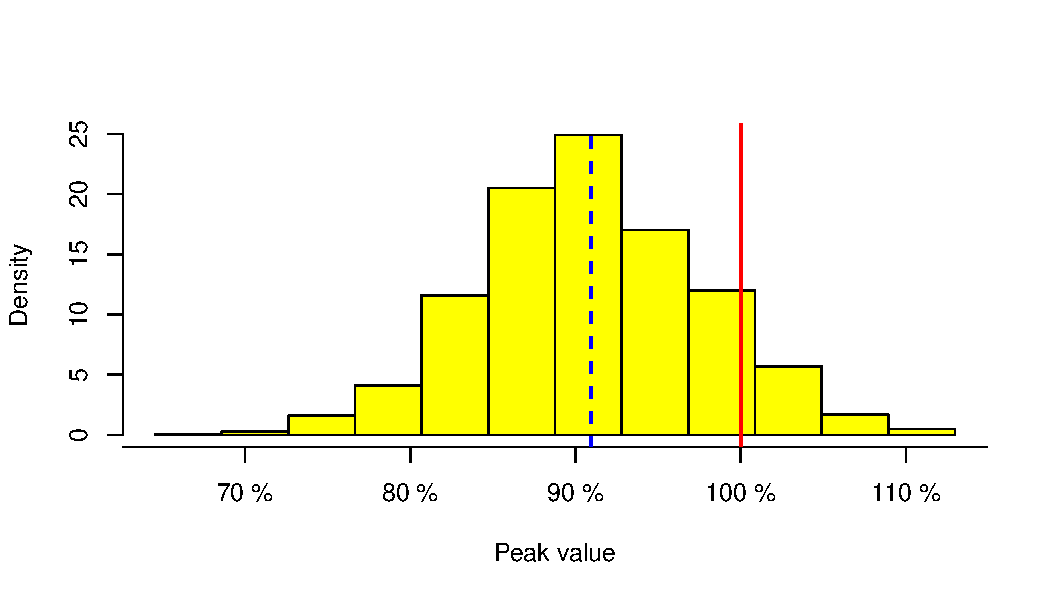
\includegraphics[width=0.5\textwidth]{peaks-hist-values-undersmooth}
        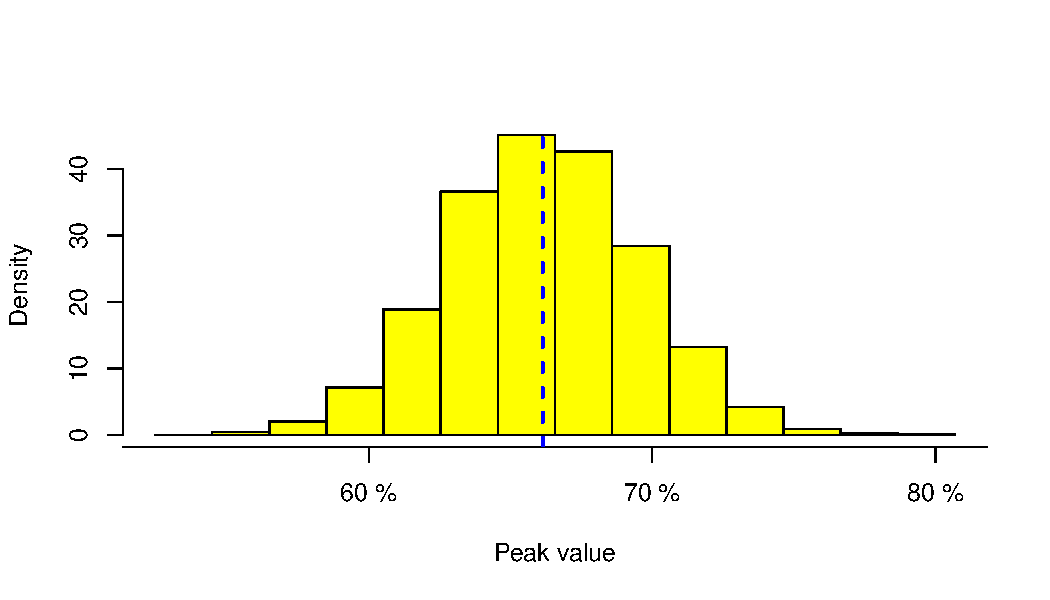
\includegraphics[width=0.5\textwidth]{peaks-hist-values-oversmooth}
     }
    \end{example}
\end{frame}

% ----- SUBSECTION: Results of the location of the peaks
\subsection{Results of the location of the peaks}
\begin{frame}\frametitle{Results of the location of the peaks}
    \footnotesize
    \begin{itemize}
        \item Average displacement of the peak: 0.833, or 3.5\% of study area diameter (small bandwidth) and 0.296 or 1.2\% (large bandwidth)
        \item Standard deviation: 0.466 or 2\% of study area diameter (small bandwidth) and 0.280 or 1.2\% (large bandwidth)
        \item 56\% of the simulations within 0.833 of the truth with the small bandwidth
        \item 46\% of the simulations within 0.296 of the truth with the large bandwidth
    \end{itemize}
    \begin{example}{\tiny{\textbf{Left:} small bandwidth. \textbf{Right:} large bandwidth. {\color{blue}Blue dashed} line is mean.}}
    \centerline{
        \label{fig:peaks-loations-hist}
        \centering
        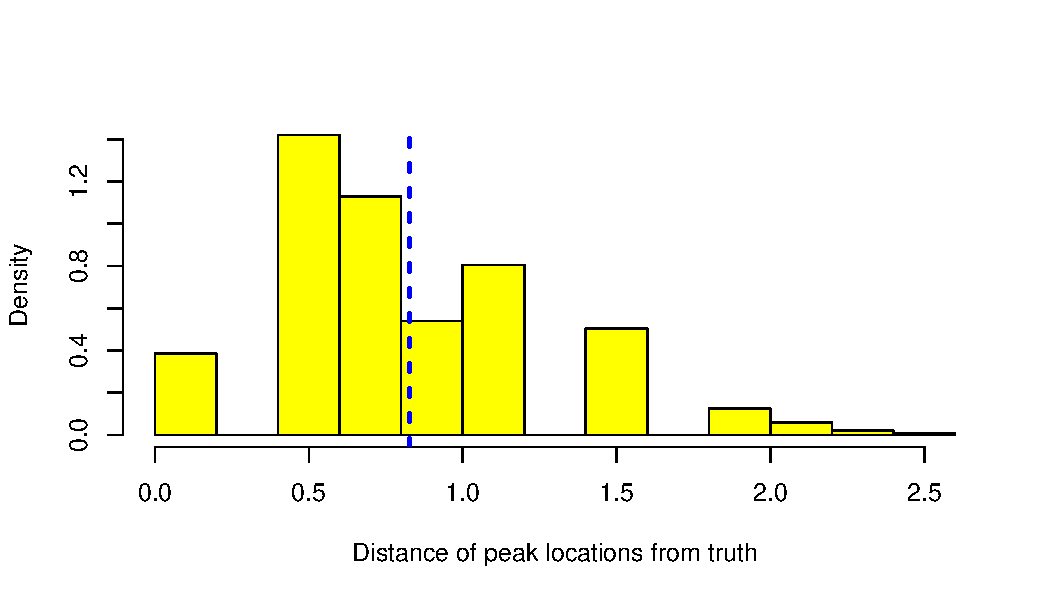
\includegraphics[width=0.5\textwidth]{peaks-hist-locations-undersmooth}
        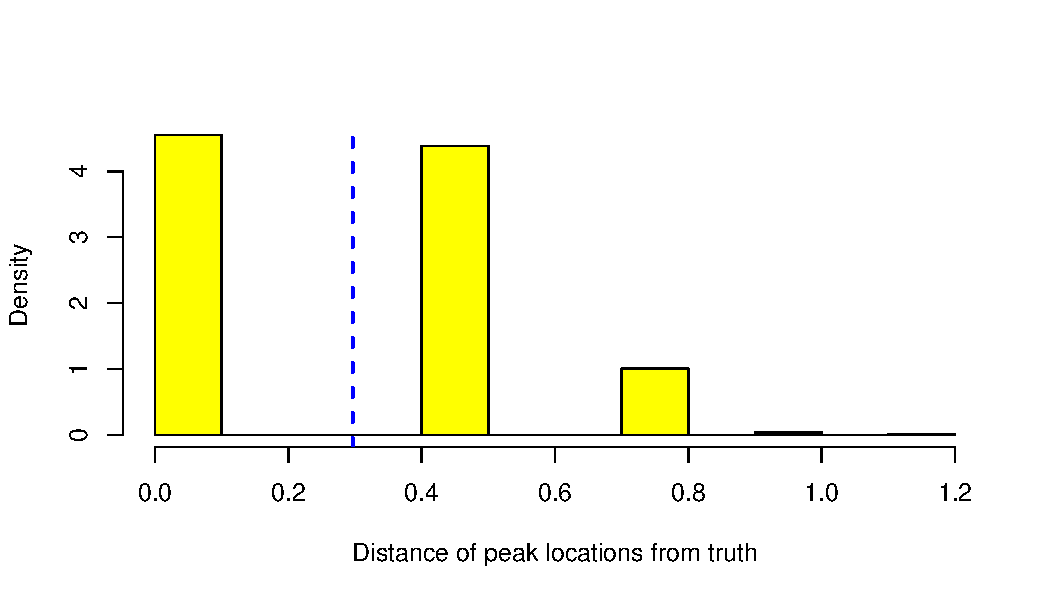
\includegraphics[width=0.5\textwidth]{peaks-hist-locations-oversmooth}
     }
    \end{example}
\end{frame}

% ----- SUBSECTION: Single peak illustration
\subsection{Single peak illustration}
\begin{frame}\frametitle{Single peak illustration}
    \begin{itemize}
        \item Peak location and height can vary
        \item DKD accuracy depends on bandwidth
    \end{itemize}
    \begin{example}{\tiny{\textbf{Left:} small value of $h$. \textbf{Right:} large value of $h$. {\color{red}*} estimated peak. \tikz\draw[blue,fill=blue] (0,0) circle (.5ex); true peak.}}
    \centerline{
        \label{fig:example-peaks}
        \centering
        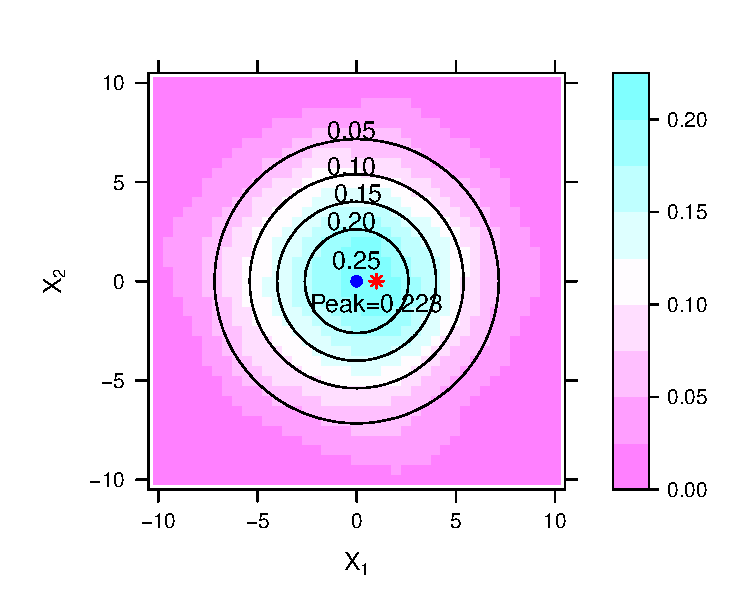
\includegraphics[width=0.5\textwidth]{example-peaks-undersmooth}
        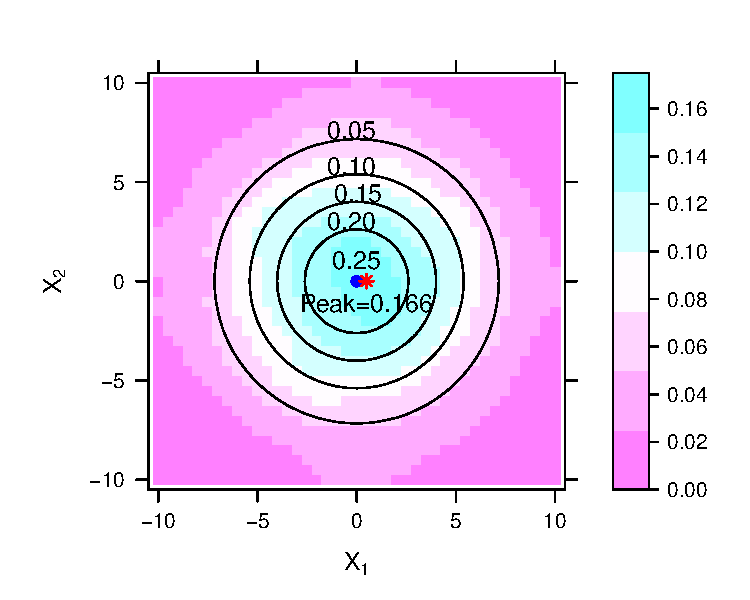
\includegraphics[width=0.5\textwidth]{example-peaks-oversmooth}
     }
    \end{example}
\end{frame}

% ----- SECTION: Conclusion
\section{Conclusion}

% ----- SUBSECTION: Conclusion
\subsection{Conclusion}
\begin{frame}\frametitle{Conclusion}
    \footnotesize
    \begin{answer}
        \begin{enumerate}[a)]
            \item
                While the MISE increased as the expected number of incidents grew,
                the normalized mean integrated squared error (NMISE) decreased at a similar rate in the examples we considered
                for Silverman ($n^{-0.741}$) and CV ($n^{-0.775}$).
                Using two years worth of data should result in the global error MISE to be about 60\% of a single year's.
                Conversely, to reduce the MISE to half of a given value one needs 2.5 times as many incidents.
            \item
                The DKD accuracy was affected by the spread of the incidence function,
                in that the MISE decreased sharply as the incidence rate spread increased and the height of the peak was lower.
                CV performed better at $\sigma^{-1.576}$ than $\sigma^{-1.421}$ for Silverman.
            \item
                By all measures, the DKD is sensitive to large variations in population density.
                For populations with a very sharp peak (10\% of the study area),
                the DKD accuracy was 2-10 times worse than all other cases.
                Otherwise the accuracy measures were stable.
                However, the estimation errors observed for the uniform populations were much lower than the peaked populations.
            \item
                Increasing the population spread saw a sharp decrease in the MISE.
        \end{enumerate}
    \end{answer}
\end{frame}

% ----- SUBSECTION: Conclusion continued
\subsection{Conclusion continued}
\begin{frame}\frametitle{Conclusion continued}
    \begin{answer}
        \begin{enumerate}[a)]
            \item
                The Normalized MISE is less than 5\% for uniform populations,
                and less than 5\% for most of the peaked populations.
                Furthermore, NMISE improves when the number of incidents increases.
                This is so regardless of whether this is due to an increase in the rate or in the population size.
                Also, the global accuracy increases when the spread of the rate increases.
            \item
                The magnitude peak can be estimated with the DKD within 10\% for uniform populations,
                but overestimates the peak for peaked populations.
            \item
                The location of the peak can be estimated with the DKD within 10\% of the size of the study area for uniform populations,
                and within 15\% for peaked populations.
        \end{enumerate}
    \end{answer}
\end{frame}

% ----- SUBSECTION: Recommendations
\subsection{Recommendations}
\begin{frame}\frametitle{Recommendations}
    \footnotesize
    \begin{recommendation}
        For computing the DKD,
        we recommend a bandwidth of between 5\% and 20\% of the width or height of the study area.
    \end{recommendation}
    \begin{recommendation}
        We recommend a sample size of at least 50 incidents for the DKD.
        For a population of size 10,000, this is an overall rate of 0.5\%,
        and for a population of size 5,000, this is an overall rate of 1.0\%.
    \end{recommendation}
    \begin{recommendation}
        For overall accuracy,
        we recommend the Silverman Rule of Thumb for computing the bandwidth due to its simplicity.
        However, if the location of the peak is important, we recommend least squares cross-validation.
    \end{recommendation}
    \begin{recommendation}
        When the population density is highly variable,
        we do not recommend computing the DKD over the entire study area.
    \end{recommendation}
\end{frame}

\subsection{Limitations}
\begin{frame}\frametitle{Limitations}
    In order to complete this research, we plan to do the following:
    \begin{itemize}
        \item Derive the \alert{optimal bandwidth} analytically
        \item \textellipsis and develop a method to estimate it accurately
        \item Vary the number of incidents: use 200, 500, and 1,000
        \item Vary the number of peaks: 1, 2, 3
        \item Use different levels of ``concentration'' of the peak by varying the standard deviation of the ``truth'': 2, 4, 8
        \item Use a non-uniform population, one that also has a peak in the center of the study area
        \item Compute the centroid of the top 5\% of the DKD values instead of the global maximum
    \end{itemize}
\end{frame}

\subsection{Further research}
\begin{frame}\frametitle{Further research}
\end{frame}

% ----- SECTION: References
\section*{References}

\begin{frame}\frametitle{References}
    \footnotesize
    \begin{thebibliography}{10}
        \bibitem[Bonita,~R., Beaglehole,~R., \& Kjellstr{\" o}m,~T., 2006]{bonita2006basic}
            Bonita,~R., Beaglehole,~R., \& Kjellstr{\" o}m,~T.
            Basic epidemiology.
            {\em World Health Organization}, 2006.
        \bibitem[Kloog, I., Haim, A., \& Portnov, B. A., 2009]{kloog2009using}
            Kloog, I., Haim, A., \& Portnov, B. A.
            Using kernel density function as an urban analysis tool: Investigating the association between nightlight exposure and the incidence of breast cancer in Haifa, Israel.
            {\em Computers, Environment and Urban Systems, 33(1), pp 55--63}, 2009.
        \bibitem[Portnov, B. A., Dubnov, J., \& Barchana, M. 2009]{portnov2009studying}
            Portnov, B. A., Dubnov, J., \& Barchana, M.
            Studying the association between air pollution and lung cancer incidence in a large metropolitan area using a kernel density function.
            {\em Socio-Economic Planning Sciences, 43(3), pp 141--150}, 2009.
        \bibitem[Zusman, M. et al., 2012.]{zusman2012residential}
            Zusman, M., Dubnov, J., Barchana, M., \& Portnov, B. A.
            Residential proximity to petroleum storage tanks and associated cancer risks: Double Kernel Density approach vs. zonal estimates.
            {\em Science of the Total Environment, 441, pp 265--276}, 2012.
    \end{thebibliography}
\end{frame}

% ----- SECTION: Thank You
\section{Thank You}

\begin{frame}
    \begin{center}
        {
            \color{orange}
            \fontsize{40}{50}\selectfont Thank You!
        }
    \end{center}
\end{frame}

\end{document}
